\chapter{A framework for analyzing the reproducibility issues of neuroimaging pipelines}\label{framework}
The Repro-tools is a framework developed for analyzing the reproducibility issues occurring in the neuroimaging pipelines. Though this framework is developed with various neuroimaging pipelines in focus, in principle, it can be also be used for analyzing data belonging to various other disciplines. The term ``condition" with respect to this framework refers to different operating systems on which the data processing takes place. Likewise, the term ``subject" with respect to this framework is used to denote the directories containing the data, that are kept under each condition. 

This chapter discusses the overall workflow of the framework, docker images, how the pipelines were encapsulated, how they were deployed, analysis of results, provenance capture and the metrics used for quantifying the differences.

%In order to analyze the results, we created a tool, which can compare the files to find differences in their checksum, called verifyFiles\footnote{\url{https://github.com/big-data-lab-team/repro-tools/blob/master/verifyFiles.py}}. 

%This tool was developed under the assumption that, under an ideal scenario, files belonging to each subject is supposed to have equal checksum under different conditions. Repro-tools help in identifying the files having differences by comparing the checksum values of files stored under different conditions. This tool can also check for corruption of files. It can compute the checksum locally and compare it against the recorded checksum (checksum recorded immediately after processing the subject) to find if the files are corrupted or not.

%It can also quantify the differences in image files with the help of metrics like Normalized root mean square error (NRMSE), Dice coefficient etc (Refer \ref{sec:num1}). Additional metrics can be configured which could be used for quantifying differences occurring in different types of files. Repro-tools can also trace the provenance of these files having the differences. It helps us identify the processes that wrote the files having differences. Provenance tracing is done with the use of data captured by Reprozip.

%Refer what is subject also in the above paragraph
%Compute Canada in architecture
\section{Repro-tools Workflow}
\begin{center}
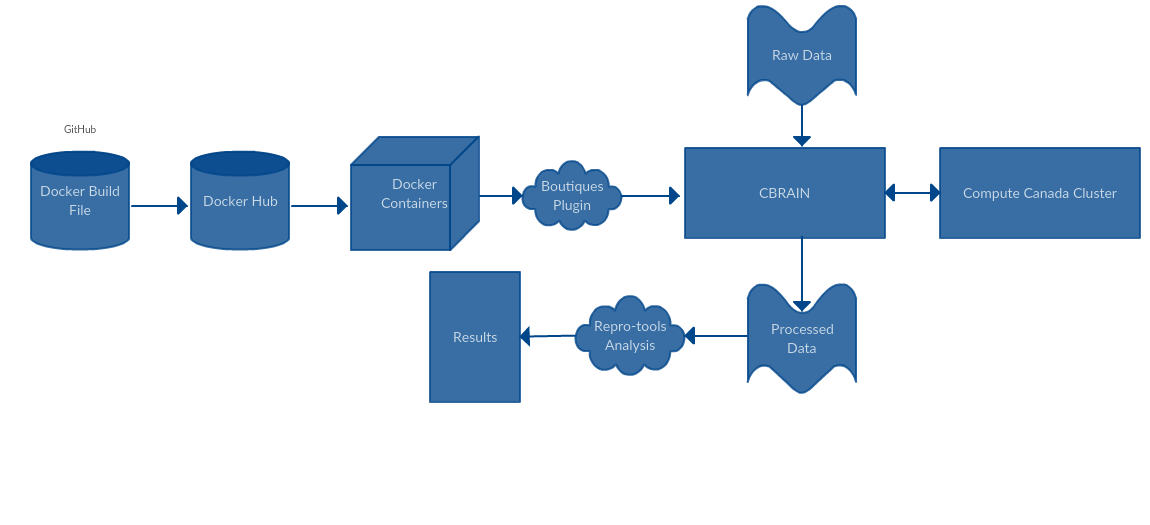
\includegraphics[width=\linewidth]{framework_architecture.png}
\captionof{figure}{Workflow of Reproducibility Analysis in neuroimaging pipelines}
\label{fig:framework_architecture}
\end{center}
\vskip 0.2in

Figure \ref{fig:framework_architecture} illustrates the overall workflow. The Docker image creation is automated. For each commit, made to the Dockerfile stored in Github\footnote{\url{https://github.com/big-data-lab-team/Dockerfiles-HCP-PreFreesurfer}}, a new build is triggered in Dockerhub\footnote{\url{https://hub.docker.com/r/bigdatalabteam/hcp-prefreesurfer/}}. These images are then used by CBRAIN for processing the subjects. Boutiques helps in deploying these containers to CBRAIN platform. CBRAIN can harness the power of computational clusters as well. The subjects processed under different conditions are then analyzed using the Repro-tools.

\section{Docker Images}
Repro-tools framework uses Docker containers for reproducibility studies. A Docker container is the running instance of a Docker image. Dockerfiles are used for specifiying the operating system and the libraries needed for creating a Docker image. With the help of automated image creation feature in Dockerhub, whenever a commit is made to the Dockerfile, a new image build gets triggered (Figure~\ref{fig:Docker_build}). Thus, the automated build makes sure that the changes are always reflected in the Docker images.

Repro-tools, before the beginning of processing a subject, makes a check to ensure that the image that is getting used is the latest one. This check makes sure that the processing is done with the up-to-date changes in the Docker images.

\begin{center}
  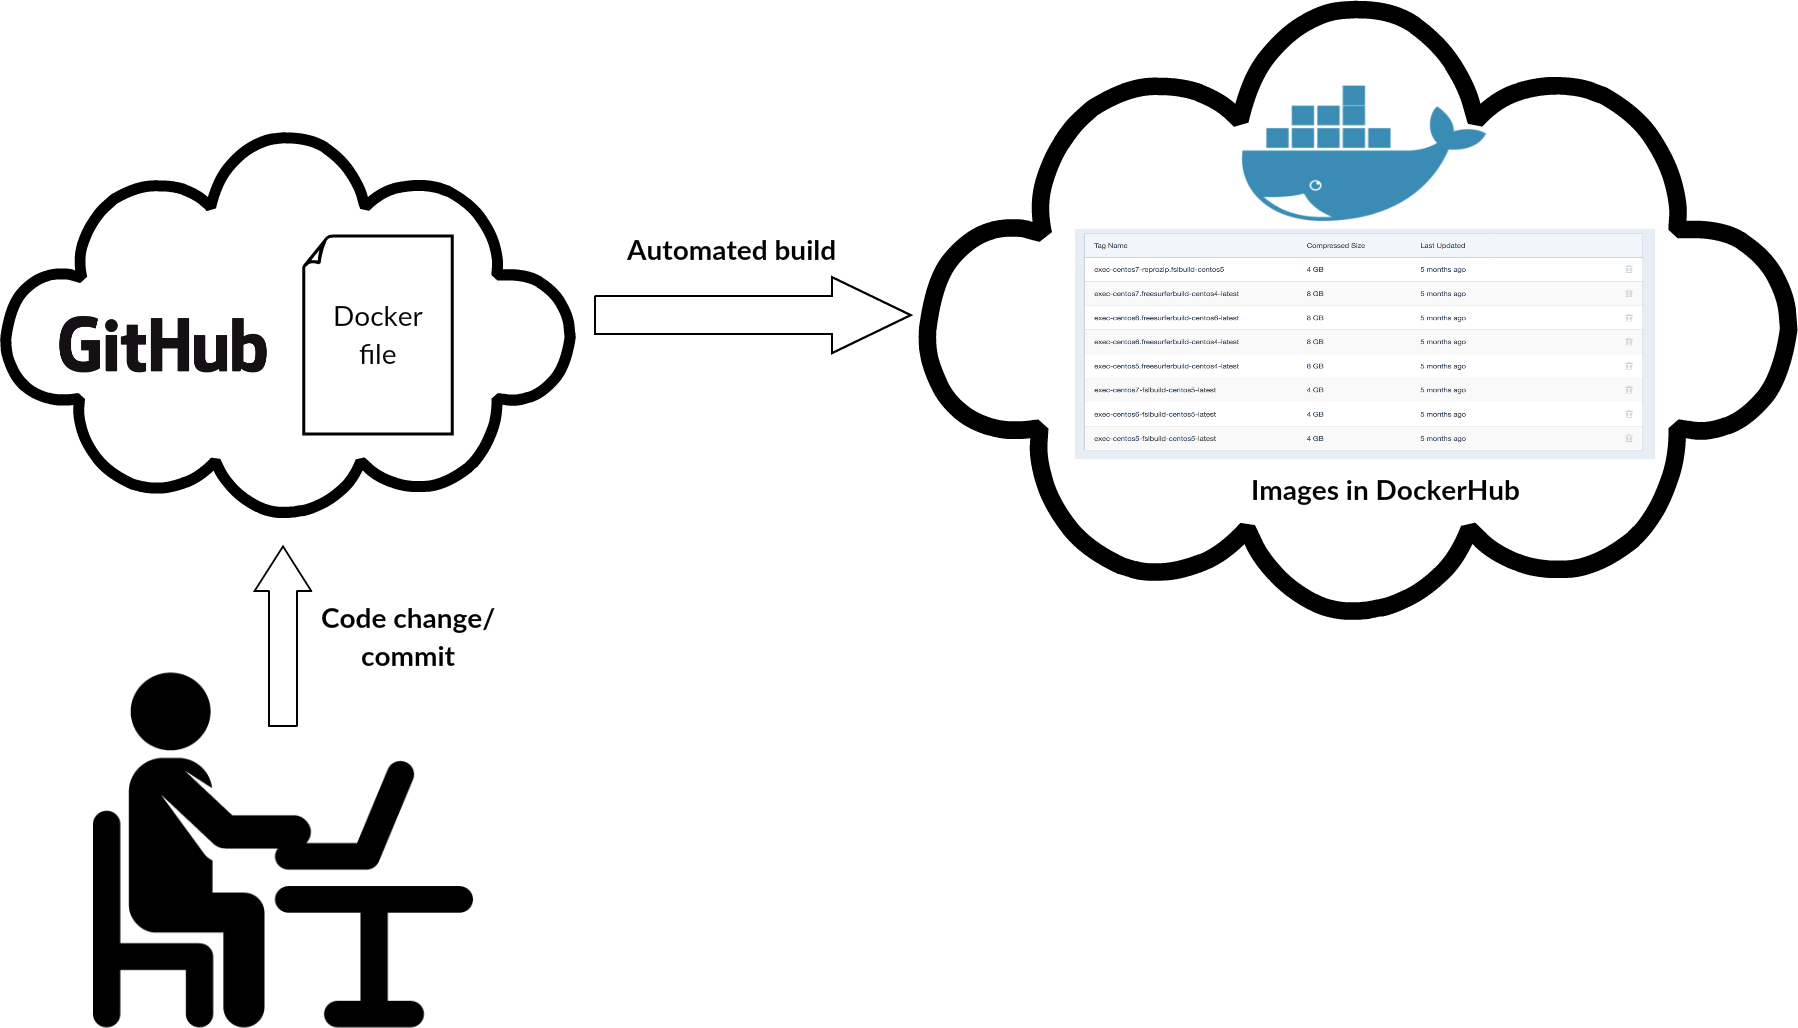
\includegraphics[width=\linewidth]{automated_build}
  \captionof{figure}{Docker automated build}
  \label{fig:Docker_build}
  \caption*{Docker logo retrieved from Docker \url{https://secure.gravatar.com/avatar/7510e100f7ebeca4a0b8c3c617349295.jpg} and GitHub logo retrieved from \url{https://github.com/logos}}
\end{center}

\section{Pipeline Encapsulation}
%Add Why wrapper and advantages
I created a wrapper script\footnote{\url{https://github.com/big-data-lab-team/Dockerfiles-HCP-PreFreesurfer/blob/master/PreFreeSurfer-DockerFiles/command-line-script.sh}} on top of the pipeline to have the features which are listed below,
\begin{itemize}
  \item Compute the checksum of the files in each subject before and after the execution
  \item Create execution directory and copy the subject to prevent corrupting the input data
  \item Record all the software (library versions) present in the container and hardware specifications of the workstation
  \item Ability to trace the execution using Reprozip (optional)
\end{itemize}

The checksums are computed before and after execution so that corruption check can be done with the use of recorded checksums. After the execution directory creation, the subject folder is copied into the execution directory and thus, it prevents the corruption of the input data. Another feature, recording of the software library versions and hardware specifications are done in order to make sure that the only factor that changes in these experiments is the operating system version. The optional Reprozip tracing feature is used to record the details of the pipeline while the processing takes place so that it can be used as a referrence for provenance tracing.

\section{Pipeline Deployment}
The Docker container containing the pipelines along with the Boutiques descriptor was deployed on a server setup as part of our study. With the help of CBRAIN along with the containers and the descriptors, we were able to process the subjects. Single server was used in order to prevent differences occurring in the files due to differences arising from the hardware architecture. Boutiques descriptors used for deploying the pipelines on CBRAIN are available at \cite{HCP_descriptors}.

%\begin{itemize}
 % \item Single server to ensure no hardware differences
  %\item Able to process multiple subjects at once
  %\item CBRAIN HCP plugins available here
%\end{itemize}

\section{File comparisons across conditions}
%Checksum
Repro-tools framework can compare the files across different conditions based on the checksum. We have used MD5\footnote{\url{https://tools.ietf.org/html/rfc1321}} algorithm for calculating the checksum of files. The output of a MD5 algorithm is a 128-bit ``fingerprint'' or ``message digest''~\cite{md5}. Though MD5 is not completely secure against collision attack, Repro-tools focus more on the data integrity than security and how fast the algorithm is able to create the checksum. These qualities make MD5 a good choice for checksum generation in Repro-tools.

Two types of differences can occur in the subjects due to the differences in the operating systems. One is inter-OS difference which occur due the operating system library updates and the other type, inter-run differences, occurs due to the pseudo-random processes used in the pipelines or due to silent crashes due to various reasons reported similiar to Table \ref{tab:table_docker}. An example of a pseudo-random process function is, a random number generator that would get initialized using a seed state. Repro-tools can be used to identify both kind of differences.

The files that are common to all the subjects only are taken into consideration for comparison. The first step is identification of files with differences in their checksums. This is identified using the checksums that are recorded after the processing. Inter-run differences are identified using the run-number added as the suffix for the conditions. For example, the two batches of subjects processed under the same condition (CentOS6) are stored as run-1 and run-2. The files belonging to the subjects stored under the above mentioned conditions are treated as inter-runs.

For the files that are identified to have differences, different kind of metrics are used base on the file type to quantify the differences. Normalized root mean square error, dice coefficient and text filter are the various metrics used for quantifying the differences. Section \ref{sec:num1} explains the metrics in detail. 

These metric values help us understand how big or small the differences are. Apart from quantifying the differences using type specific metrics, Repro-tools can also be used to trace the provenance of these differences. It is able to identify all the processes and associated parameters that wrote the files having differences. These details about various processes is helpful in debugging the pipelines. This information helps in recreating the processing step by step and also to identify the processes that creates the differences.

\newpage
\textbf{\\Algorithm 1: \underline{Algorithm for finding the file differences and metric values}\label{alg:algorithm_diff}\\}
\DontPrintSemicolon
\SetKwFunction{FMain}{\textbf{find\_differences\_and\_calculate\_metrics}}
\SetKwProg{Fn}{Function}{:}{}
\Fn{\FMain{conditions}}
{
\begin{algorithmic}[1]
\FOR{each condition C}
\FOR{each subject S}
\STATE{L\textsubscript{S,C} = list of {timestamp,file\_name,file\_size} objects, ordered by timestamp, where timestamp is the file modification time and file\_name refers to a file produced in subject S and condition C}
\ENDFOR
\ENDFOR
\FOR{each pair of conditions:C1,C2 in conditions}
  \FOR{each file name f in L\textsubscript{S,C}}
    \STATE{n\_differences[f][C1][C2] = 0} \COMMENT{Initialize the differences dictionary}
     \STATE{metric[f][C1][C2] = 0} \COMMENT{Initialize the metric value dictionary}
      \FOR{each subject S in condition C1}
        \STATE{metric[f][C1][C2][S] = 0}
        \STATE{difference = 0} \COMMENT{Variable to hold the value if file is different}
          \IF{size(f,S,C1) $\neq$ size(f,S,C2) $\parallel$ checksum(f,S,C1) $\neq$ checksum(f,S,C2)}
            \STATE{dictionary\_metrics\_value=calculate\_metric\_value(f,C1,C2,S)}
            \STATE{difference = 1}
          \ENDIF
        \STATE{n\_differences[f][C1][C2] += differ} \COMMENT{Cumulative sum of differences}
        \STATE{metric[f][C1][C2] += metric[f][C1][C2][S]} \COMMENT{Cumulative sum of metric values}
      \ENDFOR
  \ENDFOR
\ENDFOR
\end{algorithmic}
\KwRet n\_differences, metric;
}
\vskip 0.2in

Algorithm 1, Section \ref{alg:algorithm_diff} shows the high-level logic for identifying the files with differences and quantifying the differences with the help of metrices described in Section \ref{sec:num1}. First step is to get the name of all the files that are common to all the subjects and conditions. For this, we iterate through every subject in all the conditions and creates a list of files that are common to all the subjects. Along with the file\_name, we collect also the creation time, modification time etc. This list is then sorted according to the modification time. 

A pair of condition is taken at a time as the following step (Line 6). The files under the subject in two different conditions are then comapred to see if their file sizes or checksums differ (Line 13). If a difference is observed, then the metric value is computed it is stored in a dictionary with the file name, subject and condition as the key value. The difference in the file is denoted with a value ``1" into a variable (Lines 14-15).

%\section{Metrics calculation using Apache Spark}
%In order to parallelize the analysis and metric calulation and to harness the power of high performance computing power (Compute Canada), an Apache Spark based variant of verifyFiles script was created\footnote{\url{https://github.com/lalet/Big-Data-Spark}}. Parallelized analysis and metrics calculation could reduce the time taken for analysis considerably. The sequence of steps followed in the Apache Spark function is described below,
%\begin{enumerate}
 % \item Map a pair of files along with its checksum
  %\item Check if the checksums are equal
  %\item If they are not equal compute the metric associated with the type of file
  %\item Reduce the values using filenames as the key
  %\item Write the keys and values to a csv file
%\end{enumerate}

%Add brief description about Map and reduce

\section{Provenance Capture}
Repro-tools traces the provenance of differences using the data captured by Reprozip. Reprozip records the data in an SQLite\footnote{\url{https://www.sqlite.org/}} database. Repro-tools framework queries this database to find out the provenance information about the files that has a difference in their checksum. Figure \ref{fig:provenance-query} contains the query used for finding the provenance information.\\

%Add the tracing command example
\begin{tcolorbox}[colback=black!5!white,colframe=black!75!black]
SELECT DISTINCT executed\_files.name, executed\_files.argv, executed\_files.envp, executed\_files.timestamp, executed\_files.workingdir from executed\_files INNER JOIN opened\_files where opened\_files.process = executed\_files.process and opened\_files.name like ? and opened\_files.mode=2 and opened\_files.is\_directory=0',('\%/'+file\_name,)
\end{tcolorbox}
\captionof{figure}{Query for provenance information}
\label{fig:provenance-query}

Query above returns us the details about the 1) processes that wrote the file; 2) command line arguments used by those processes; 3) Environment variables used; 4) timestamp; 5) working directory. By the help of query shown in Figure \ref{fig:provenance-query} and its output from the Reprozip database, we can identify the processes in the pipeline that create these differences.

\section{Metrics} \label{sec:num1}
The metrics that are used to quantify the differences are described below.

\subsection{Normalized Root Mean Square Error (NRMSE)}
The Root Mean Square Deviation (RMSD) or root-mean-square error (RMSE), according to~\cite{khosrow2017handbook} is, ``a frequently used measure of the difference between values predicted by a model or an estimator and the values actually observed". Normalizing the RMSD value makes it easier to compare between models or datasets. The equation for NRMSE is shown in equation~\ref{eq_one}.

\begin{equation}
  \label{eq_one}
    NRMSE = \frac{\sqrt{mean\_square\_difference}}{maximum\_intensity - minimum\_intensity}
\end{equation}

\iffalse
\hrulefill
\caption*{\textbf{Algorithm 2:} Algorithm for finding the normalized root mean square value}
\label{alg:algorithm_diff}
\hrulefill

\DontPrintSemicolon
\SetKwFunction{FMain}{Convert\_image}
\SetKwProg{Fn}{Function}{:}{}
\Fn{\FMain{$image$}}{
  \begin{algorithmic}[1]
    \IF{image extension is ``.mgz":}
      \STATE convert image to ``.nii"
    \ELSE
      \STATE do nothing
    \ENDIF
  \end{algorithmic}
\KwRet image\;
}
\hfill \break
\hfill \break
\SetKwFunction{FNrmse}{Get\_NRMSE}
\SetKwProg{Pn}{Function}{:}{}
\Pn{\FNrmse{$image\-1$,$image\-2$}}{
  \begin{algorithmic}[1]
    \STATE image\_1 $\leftarrow$ Convert\_image(image\-1);
    \STATE image\_2 $\leftarrow$ Convert\_image(image\-2);
    \STATE minimum\_intensity $\leftarrow$ get the min. intensity value from image\_1; \COMMENT{using FSL}
    \STATE maximum\_intensity $\leftarrow$ get the max. intensity value from image\_1;
    \STATE \textbf{fslmaths} image\-1 \text{-sub} image\-2 \text{-sqr} $\rightarrow$ diff; \COMMENT{computing the mean square difference using FSL}
    \STATE meandifference $\leftarrow$ \textbf{fslstats} diff -m ; \COMMENT{get the mean square difference}
    \STATE \textbf{NRMSE} $\leftarrow$ $\sqrt{\frac{mean\_difference}{maximum\_intensity-minimum\_intensity}}$; \COMMENT{Normalized root mean square error value}
  \end{algorithmic}
\KwRet NRMSE\;
}
\fi

\subsection{Dice Similarity Coefficient}
Dice Similarity Coefficient~\cite{ECY:ECY1945263297} can be used as a statistical validation metric for measuring the reproducibility of magnetic resonance images~\cite{Zou2004}. To measure the similarity of image files in reproducibility study, we used dice similarity coefficient. The coefficient ranges from [0.0,1.0]. 1.0 meaning the images are exactly similiar and 0 meaning there is zero similarity. The equation used for finding the dice coefficient is given in \ref{eq:eq_two}. Consider I1 \& I2, as non-zero voxels from two images.

\begin{equation}
  \label{eq:eq_two}
    Dice\_coefficient = \frac{((|I1| + |I2|) - (2|I1 - I2|))}{(|I1| + |I2|)}
\end{equation}

\iffalse
\DontPrintSemicolon
\SetKwFunction{FMain}{Convert\_image}
\SetKwProg{Fn}{Function}{:}{}
\Fn{\FMain{$image$}}{
  \begin{algorithmic}[1]
    \IF{image extension is ``.mgz":}
      \STATE convert image to ``.nii"
    \ELSE
      \STATE do nothing
    \ENDIF
  \end{algorithmic}
\KwRet image\;
}
\hfill \break
\hfill \break
\SetKwFunction{FDice}{Get\_NRMSE}
\SetKwProg{Pn}{Function}{:}{}
\Pn{\FDice{$image\-1$,$image\-2$}}{
  \begin{algorithmic}[1]
    \STATE image\_1 $\leftarrow$ Convert\_image(image\-1);
    \STATE image\_2 $\leftarrow$ Convert\_image(image\-2);
    \STATE \textbf{fslmaths} image\_1 \text{-sub} image\_2 $\rightarrow$ diff;
    \STATE nonzero\_voxels\_image1 $\leftarrow$ get the $\textless$non-zero voxels$\textgreater$ $\textless$volume$\textgreater$ from image\_1; \COMMENT{using FSL}
    \STATE nonzero\_voxels\_image2 $\leftarrow$ get the $\textless$non-zero voxels$\textgreater$ $\textless$volume$\textgreater$ from image\_2;
    \STATE nonzero\_voxels\_difference $\leftarrow$ get the $\textless$non-zero voxels$\textgreater$ $\textless$volume$\textgreater$ from difference of images;
    \STATE \textbf{Dice\_coeff} $\leftarrow$ $\frac{(nonzero\_voxels\_image1+nonzero\_voxels\_image2)-nonzero\_voxels\_difference}{(nonzero\_voxels\_image1+nonzero\_voxels\_image2)}$;
  \end{algorithmic}
\KwRet \textbf{Dice\_coeff}\;
}
\caption*{Algorithm 2: Algorithm for finding Dice coefficient similarity from images}
\label{alg:dice_algorithm}
\fi

\subsection{Text Filtering}
Since the hardware architecture used for processing the neuroimages has an effect on the output images~\cite{10.1371/journal.pone.0038234}, text filtering is done in order to make sure that, the hardware specifications remains the same throughout the experiment. The wrapper script around the HCP preprocessing pipelines records the hardware specification of the machine on which the subject gets processed. This recorded text file contains the details about the processor, vendor\_id, cpu family, model name etc. With the help of these details, text filtering metric return a '0' if the records are equal and '1' if any of these details are found to be different. This metric is more ideal in cas of a study that uses high performance cluster with heterogeneous machines for processing the data. For this study, we used a single sever to maintain the homogeneity of the processing environment.
